\documentclass[10pt,twocolumn,letterpaper]{article}

\usepackage{cvpr}
\usepackage{times}
\usepackage{epsfig}
\usepackage{graphicx}
\usepackage{amsmath}
\usepackage{amssymb}
\usepackage[
natbib=true,
style=numeric,
sorting=none
]{biblatex}
\addbibresource{egbib.bib}

% Include other packages here, before hyperref.

% If you comment hyperref and then uncomment it, you should delete
% egpaper.aux before re-running latex.  (Or just hit 'q' on the first latex
% run, let it finish, and you should be clear).
\usepackage[breaklinks=true,bookmarks=false]{hyperref}

\cvprfinalcopy % *** Uncomment this line for the final submission

\def\cvprPaperID{****} % *** Enter the CVPR Paper ID here
\def\httilde{\mbox{\tt\raisebox{-.5ex}{\symbol{126}}}}

% Pages are numbered in submission mode, and unnumbered in camera-ready
%\ifcvprfinal\pagestyle{empty}\fi
\setcounter{page}{1}
\begin{document}

%%%%%%%%% TITLE
\title{Crowd counting on fixed camera images}

\author{Pierpaolo D'Odorico\\
{\tt\small pierpaolo.dodorico@studenti.unipd.it}
\and
Massimiliano Conte\\
{\tt\small massimiliano.conte@studenti.unipd.it}
}


\maketitle
%\thispagestyle{empty}
\begin{abstract}



In this work we compared different computer vision tecniques in order to estimate the number of people in a frame. The counting is performed on images captured from a fixed camera placed in a shopping mall. Some applications of this kind of counting on a static view are security and safety tasks, estimating the number of visitors on a mall for a/b testing purpose, planning spaces and services or verify compliance with covid-19 social distancing.

\end{abstract}

%%%%%%%%% BODY TEXT
\section{Introduction}

The crowd counting problem received a lot of attention in recent years, due to its direct connection with crowd control and public safety. For this reason many techniques were recently proposed.
Our idea is to compare two main tecniques in this fixed camera setting, one that is fast to implement and the other one more challenging, in order to verify if it is worth it to spend time for a more sophisticated solution. The first approach is to direcly estimate the number of people performing regression with a deep convolutional neural network, such as the VGG16 network \cite{simonyan2014very}. We chose this very deep network since it is easy to handle for our purposes, unlike more complex architectures that have, for example, skip layer connections, and also because it is the base for the second technique. The second approach performs an undirect estimate of the number of people. First it is estimated the density of people in the image, then starting from the obtained density map the count is inferred. This second approach represents the base idea for the state of the art methods in croud counting, where images could have a completely different number of people on  differents enviroment and perspective. After implementing the two approaches on our problem, we found that a simple regression based on neural networks could perform as good as density based approach, probably exploiting the fixed background.


%------------------------------------------------------------------------
\section{Related work}

\subsection{VGG net}
We based our work on information contained in different papers about computer vision tasks and crowd counting. The first one is related to the base network of both approaches, the VGG16 net \cite{simonyan2014very}. In this paper the authors investigated the effect of a deeper (with respect to previous architectures) convolutional neural network on the classification accuracy in the
large-scale image recognition setting, specifically on the \textit{imageNet} dataset \cite{deng2009imagenet}. In this convolutional neural networks they used very small (3x3) convolution filters, which have shown a significant improvement on the prior state of the art configurations. They also pushed the depth to 16-19 weight layers (Fig.\ref{fig:vgg16}). Those convolutional filters learned during \textit{imageNet} classification task can be useful in our application, giving a meaningful feature extraction for finding people in images.

\begin{figure}[h!]
  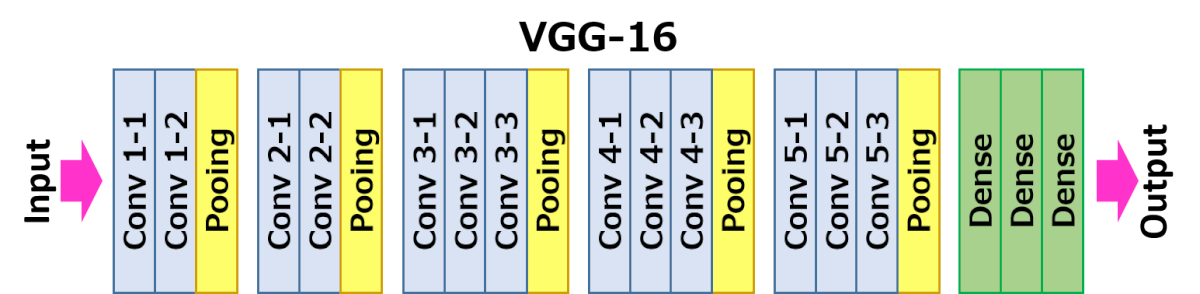
\includegraphics[width=\linewidth]{pics/vgg16.png}
  \caption{VGG16 deep CNN architecture.}
  \label{fig:vgg16}
\end{figure}

\subsection{Density based approach}
The crowd counting based on density map estimation is a well known approach. One solution that is robust with respect to a variety of image properties is the \textit{Multi-Column Convolutional Neural Network (MCCNN)} \cite{zhang2016single}. The authors designed a system capable of detecting heads of different sizes, both in dense or sparse situations. Their work is first based on the generation of ground-truth density maps via geometry-adaptive kernels, for handling both dense and sparse images. Their architecture is designed in such a way that is able to detect heads of different sizes, in particular they built a neural network with three branches, one for head size, small, medium and large heads. For the training they pre trained separately each branch, and then the full network. The output of the network was designed and trained to be the estimation of the ground truth density maps. In order to train such a network, since are required ground truth density maps, a datatset with head annotations is a requisite, and for this reason they also introduced \textit{Shanghai-tech}, a new large scale crowd counting dataset. 

\begin{figure}[h!]
	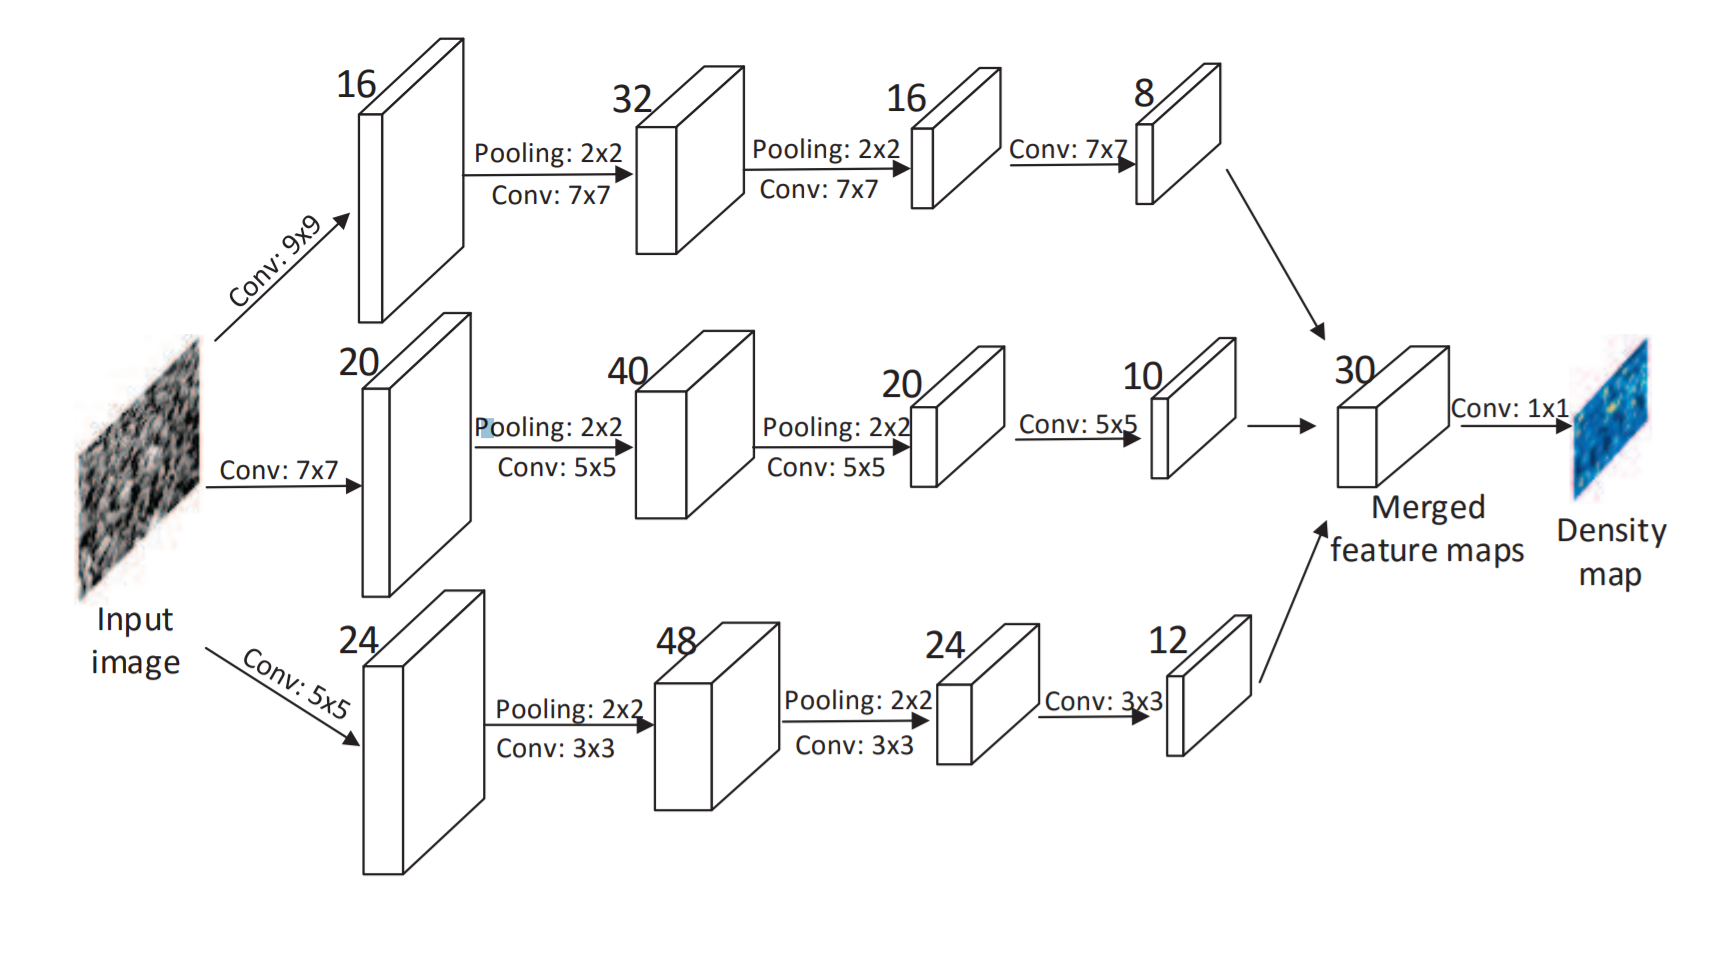
\includegraphics[width=\linewidth]{pics/MCCNN.png}
	\caption{MCCNN architecture.}
	\label{fig:MCCNN}
\end{figure}


 The models that we implemented are related to a more recent paper that simplifies the convolutional neural network of the previous work, by removing the multy-branch structure and going further with the deepness. They also experimented with the stride of convolutions, in an architecture they called \textit{CSRNet} \cite{li2018csrnet}. Designing a model which is automatically able to distinguish heads of different sizes achieved better results with respect to \textit{MCCNN}. This architecture is basically the \textit{VGG16} net (without the classifier), with other convolutional layers on top of it. For the training they fine tuned the network, starting from \textit{ImageNet} learned weights for the $VGG16$ part and random normal initialization for the others. Since those methods \cite{zhang2016single,li2018csrnet} don't use dense layers, they can work with images of any size.

\begin{figure}[h!]
	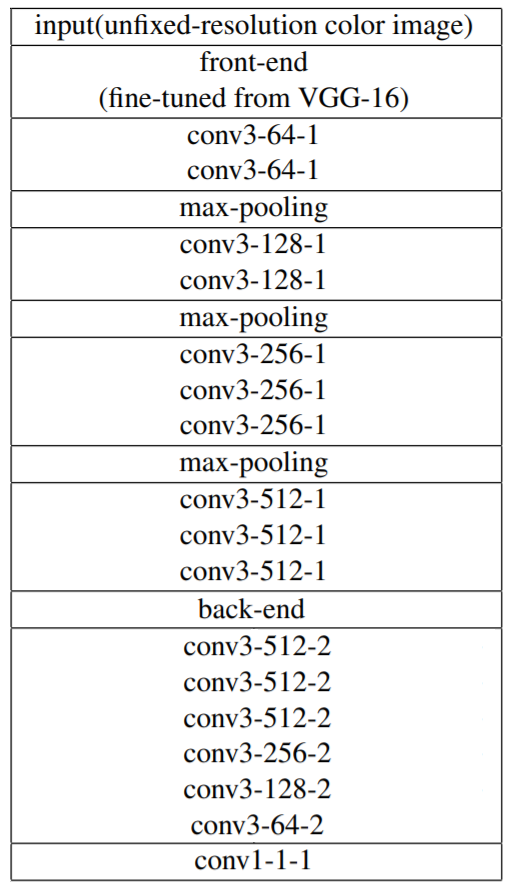
\includegraphics[width=0.5\columnwidth]{pics/CSRnet.png}
	\centering
	\caption{Best CSRnet architecture\\ numbers are: kernel size - \# of filters - stride.}
	\centering
	\label{fig:CSRnet}
\end{figure}



%------------------------------------------------------------------------
\section{Datasets}
\subsection{Mall dataset}
\subsection{Shanghai tech dataset}

jdbfjdbjfbfdbfsdjb

\printbibliography

%{\small
%\bibliographystyle{ieee_fullname}
%\bibliography{egbib}
%}

\end{document}
